% ------------------------------------------------------------------
% Algebra Extension booklet.
% GENERATED by src/build.py from src/content_extension.py -- edit content_extension.py and
% re-run the build, so every practice answer gets re-checked.
% ------------------------------------------------------------------
\documentclass[12pt,a4paper]{article}
\usepackage[a4paper,top=1.4cm,bottom=1.8cm,left=1.5cm,right=1.5cm,footskip=0.8cm]{geometry}
\usepackage[T1]{fontenc}
\usepackage[scaled=0.95]{helvet}
\renewcommand{\familydefault}{\sfdefault}
\usepackage{amsmath,amssymb}
\usepackage[table]{xcolor}
\usepackage[most]{tcolorbox}
\usepackage{enumitem,multicol,array,tabularx,pifont,fancyhdr,titlesec}

\definecolor{accent}{HTML}{1D6B8C}
\definecolor{accentlight}{HTML}{E3F0F6}
\definecolor{checkcol}{HTML}{8A3B12}
\definecolor{checklight}{HTML}{F6E7DE}
\definecolor{muted}{HTML}{56616B}
\definecolor{good}{HTML}{2E7D32}
\definecolor{warm}{HTML}{FFF6DD}
\definecolor{warmedge}{HTML}{E3B341}

\setlength{\parindent}{0pt}
\setlength{\parskip}{4pt}
\newcommand{\cmark}{\textcolor{good}{\ding{51}}}
\newcommand{\xmark}{\textcolor{red!70!black}{\ding{55}}}
\newcommand{\tickbox}{{\Large$\square$}}
\titleformat*{\subsection}{\large\bfseries\color{accent}}
\titlespacing*{\subsection}{0pt}{8pt}{4pt}

\pagestyle{fancy}
\fancyhf{}
\renewcommand{\headrulewidth}{0pt}
\fancyfoot[L]{\footnotesize\color{muted}Algebra Extension}
\fancyfoot[R]{\footnotesize\color{muted}Page \thepage}

% --- boxes -----------------------------------------------------------------
\tcbset{base/.style={enhanced, arc=2mm, boxrule=0.8pt, left=3mm, right=3mm, top=1.5mm, bottom=1.5mm}}
\newtcolorbox{tipbox}[1]{base, fontupper=\large, colframe=accent, colback=white, before upper={\textbf{#1.}\ }}
\newtcolorbox{stepsbox}[1]{base, fontupper=\large, colframe=accent, colback=white, before upper={\textbf{#1}\par}}
\newtcolorbox{rememberbox}{base, fontupper=\large, colframe=warmedge, colback=warm, before upper={\textbf{Remember:}\ }}
\newenvironment{examples}{\begin{tcbraster}[raster columns=3, raster equal height=rows,
  raster column skip=2.5mm, raster row skip=2.5mm, raster before skip=2mm, raster after skip=3mm]}{\end{tcbraster}}
\newcommand{\example}[3]{\begin{tcolorbox}[base, colframe=black!25, colback=white, boxrule=0.5pt, arc=1.5mm]
  {\Large #1}\par\vspace{-2pt}{\color{black!25}\rule{\linewidth}{0.4pt}}\par
  {\normalsize\color{black!75}#2}\par\vspace{2pt}
  {\Large\color{good}\boldmath #3}\end{tcolorbox}}

\newcommand{\stepnum}[2]{\tikz[baseline=(n.base)]\node[circle,fill=#2,text=white,inner sep=0pt,
  minimum size=8mm,font=\large\bfseries](n){#1};}
\newcommand{\qnum}[1]{\tikz[baseline=(n.base)]\node[circle,fill=accentlight,text=accent,inner sep=0pt,
  minimum size=6mm,font=\small\bfseries](n){#1};}
\newcommand{\cnum}[1]{\tikz[baseline=(n.base)]\node[circle,fill=checklight,text=checkcol,inner sep=0pt,
  minimum size=6.5mm,font=\small\bfseries](n){#1};}

% \banner{number}{title}{label}{colour}
\newcommand{\banner}[4]{\begin{tcolorbox}[enhanced, colback=#4, colframe=#4, arc=2mm,
  left=3mm, right=3mm, top=2mm, bottom=2mm, after skip=3mm]
  \color{white}\tikz[baseline=(n.base)]\node[circle,fill=white,text=#4,inner sep=0pt,
  minimum size=8.5mm,font=\Large\bfseries](n){#1};\hspace{3mm}{\LARGE\bfseries #2}\hfill
  \colorbox{white!20!#4}{\bfseries\MakeUppercase{#3}}\end{tcolorbox}}

% \qbox{n}{question}{height}
\newcommand{\qbox}[3]{\begin{tcolorbox}[base, height=#3, text fill, colframe=black!30, colback=white, boxrule=0.5pt,
  arc=1.5mm, top=1.5mm, bottom=2mm]\qnum{#1}\hspace{2.5mm}{\Large #2}\par\vfill
  {\Large$=$}\hspace{2mm}\textcolor{black!45}{\rule{0.8\linewidth}{0.6pt}}\end{tcolorbox}}

% \cbox{n}{question}{height}  -- skill check question, with a mark box
\newcommand{\cbox}[3]{\begin{tcolorbox}[base, height=#3, text fill, colframe=checkcol!70, colback=white, boxrule=0.8pt,
  arc=1.5mm, left=2mm, right=2mm, top=1.5mm, bottom=2mm]\cnum{#1}\hfill
  \fcolorbox{checkcol}{white}{\rule{0pt}{4.5mm}\hspace{4.5mm}}\par\vspace{1mm}
  {\large #2}\par\vfill
  {\large$=$}\hspace{1mm}\textcolor{black!45}{\rule{0.8\linewidth}{0.6pt}}\end{tcolorbox}}

% \checkhead{n}{title}{instruction}{marks}
\newcommand{\checkhead}[4]{\begin{tcolorbox}[enhanced, colback=checklight, colframe=checklight, arc=1.5mm,
  left=2mm, right=2mm, top=0.8mm, bottom=0.8mm, before skip=4mm, after skip=2mm]
  \cnum{#1}\hspace{2mm}\textbf{\color{checkcol}#2}\quad #3\hfill
  \textbf{\color{checkcol}Mark: \underline{\hspace{8mm}} / #4}\end{tcolorbox}}

\newcommand{\fillline}[1]{\textcolor{black}{\rule{#1}{0.6pt}}}
\newcommand{\ansline}[1]{\textcolor{black!45}{\rule{#1\linewidth}{0.6pt}}}

% \pbox[options]{n}{height}{body} -- a practice question of any type
\newcommand{\pbox}[4][]{\begin{tcolorbox}[base, height=#3, text fill, colframe=black!30, colback=white, boxrule=0.5pt,
  arc=1.5mm, top=1.5mm, bottom=2mm, #1]\qnum{#2}\hspace{2.5mm}#4\end{tcolorbox}}
% \kbox[options]{n}{height}{body} -- a skill check question of any type, with a mark box
\newcommand{\kbox}[4][]{\begin{tcolorbox}[base, height=#3, text fill, colframe=checkcol!70, colback=white, boxrule=0.8pt,
  arc=1.5mm, left=2mm, right=2mm, top=1.5mm, bottom=2mm, #1]\cnum{#2}\hfill
  \fcolorbox{checkcol}{white}{\rule{0pt}{4.5mm}\hspace{4.5mm}}\par\vspace{1mm}#4\end{tcolorbox}}

\begin{document}

\thispagestyle{empty}
\begin{tcolorbox}[enhanced, colback=accent, colframe=accent, arc=3mm, halign=center, top=12mm, bottom=11mm]
\color{white}{\small\bfseries E\,X\,T\,E\,N\,S\,I\,O\,N\quad W\,O\,R\,K\,B\,O\,O\,K}\par\vspace{3mm}
{\fontsize{34}{40}\selectfont\bfseries Algebra Extension}\par\vspace{3mm}
{\Large Take your algebra to the next level.}
\end{tcolorbox}
\vspace{10mm}
{\large Name: \fillline{9.5cm} \hfill Class: \fillline{3.5cm}}

\vspace{12mm}
{\Large\bfseries\color{accent} My progress}\par\vspace{2mm}
\renewcommand{\arraystretch}{2.1}
\begin{tabularx}{\linewidth}{|c|X|c|p{2.4cm}|}
\hline
\rowcolor{accentlight} & \textbf{Skill} & \small\textbf{Practice done} & \small\textbf{Skill Check} \\ \hline
\textbf{\color{accent}\large 1} & \textbf{Factorising Fully}\newline {\small\color{muted}I can take out the highest common factor, e.g. $12x^{2} + 30x = 6x(2x + 5)$} & \tickbox & \hfill/\,4 \\ \hline
\textbf{\color{accent}\large 2} & \textbf{Substituting Negatives}\newline {\small\color{muted}I can substitute negative numbers, e.g. if $x = -3$ then $x^{2} - 2x = 15$} & \tickbox & \hfill/\,4 \\ \hline
\textbf{\color{accent}\large 3} & \textbf{Index Laws}\newline {\small\color{muted}I can use the index laws and explain them, e.g. $3^{4} \times  3^{2} = 3^{6}$} & \tickbox & \hfill/\,3 \\ \hline
\textbf{\color{accent}\large 4} & \textbf{Equations with Brackets}\newline {\small\color{muted}I can solve equations like $3(x + 4) = 27$, and write equations from a story} & \tickbox & \hfill/\,3 \\ \hline
\textbf{\color{accent}\large 5} & \textbf{Inequalities}\newline {\small\color{muted}I can solve an inequality and show it on a number line, e.g. $2x + 3 < 11$ gives $x < 4$} & \tickbox & \hfill/\,2 \\ \hline
\textbf{\color{accent}\large 6} & \textbf{Writing Linear Rules}\newline {\small\color{muted}I can write a rule like $y = 2x + 3$ from a table of values or a story} & \tickbox & \hfill/\,2 \\ \hline
\multicolumn{3}{r|}{\textbf{Skill Check total}} & \hfill/\,18 \\ \cline{4-4}
\end{tabularx}
\newpage
\banner{1}{Factorising Fully}{Learn}{accent}
\begin{tcolorbox}[enhanced, colback=accentlight, colframe=accent, boxrule=0pt, leftrule=1.5mm, arc=0mm, top=1.5mm, bottom=1.5mm]\textbf{Goal:} I can take out the highest common factor, e.g. $12x^{2} + 30x = 6x(2x + 5)$\end{tcolorbox}
\large

\textbf{Factorising fully} means taking out the \textbf{highest common factor} (HCF):
the \textbf{biggest number} and \textbf{any letters} that go into every term.

\begin{tipbox}{The common mistake}
$12x + 36 = 6(2x + 6)$ is \textbf{not} fully factorised --- look inside the bracket:
$2x$ and $6$ still have a common factor of 2. Taking out 12 straight away gives $12(x + 3)$.
\end{tipbox}

\begin{stepsbox}{How to factorise fully}
\begin{enumerate}[nosep]
\item \textbf{Numbers:} find the HCF. Try the \textbf{smaller} number first --- does it divide the other one? If not, try its next-biggest factor.
\item \textbf{Letters:} if \textbf{every} term has the same letter, take it out too (the lowest power).
\item \textbf{Divide} each term by the HCF and write the results in the bracket.
\item \textbf{Check:} nothing in the bracket shares a factor any more, and expanding gives the question.
\end{enumerate}
\end{stepsbox}

\subsection*{Worked examples}
\begin{examples}
\example{$12x + 36$}{12 goes into 36, so the HCF is 12\\$12x \div  12 = x$, $36 \div  12 = 3$}{$= 12(x + 3)$}
\example{$18a - 24$}{18 doesn't go into 24; 6 does\\$18a \div  6 = 3a$, $24 \div  6 = 4$}{$= 6(3a - 4)$}
\example{$12x^{2} + 30x$}{Numbers: HCF is 6\\Letters: both have $x$}{$= 6x(2x + 5)$}
\example{$8ab + 12a$}{Numbers: HCF is 4\\Letters: both have $a$}{$= 4a(2b + 3)$}
\example{$15x^{2} - 25x$}{Numbers: HCF is 5\\Letters: both have $x$}{$= 5x(3x - 5)$}
\example{$14xy + 21y$}{Numbers: HCF is 7\\Letters: both have $y$}{$= 7y(2x + 3)$}
\end{examples}

\begin{rememberbox}
$12x^{2} + 30x = 6(2x^{2} + 5x)$ is only \textbf{partly} factorised: $2x^{2}$ and $5x$ both still have an $x$.
Always look inside your bracket before you stop.
\end{rememberbox}

\newpage\normalsize
\banner{1}{Factorising Fully}{Practice}{accent}
{\large\textbf{Factorise fully.}} {\color{muted}Show your working in each box.}\par\vspace{1mm}
\begin{tcbraster}[raster columns=2, raster column skip=4mm, raster row skip=3mm]
\qbox{1}{$10x + 30$}{3.45cm}
\qbox{2}{$16a - 24$}{3.45cm}
\qbox{3}{$18y + 27$}{3.45cm}
\qbox{4}{$24x - 36$}{3.45cm}
\qbox{5}{$20m + 50$}{3.45cm}
\qbox{6}{$42 - 28x$}{3.45cm}
\qbox{7}{$x^{2} + 9x$}{3.45cm}
\qbox{8}{$6x^{2} + 9x$}{3.45cm}
\qbox{9}{$10a^{2} - 15a$}{3.45cm}
\qbox{10}{$16x^{2} + 24x$}{3.45cm}
\qbox{11}{$9ab + 12a$}{3.45cm}
\qbox{12}{$20xy - 30y$}{3.45cm}
\end{tcbraster}
\vfill\centerline{\color{good}\bfseries \ding{51}\ Check your answers at the back. Fix any you got wrong.}
\newpage
\banner{2}{Substituting Negatives}{Learn}{accent}
\begin{tcolorbox}[enhanced, colback=accentlight, colframe=accent, boxrule=0pt, leftrule=1.5mm, arc=0mm, top=1.5mm, bottom=1.5mm]\textbf{Goal:} I can substitute negative numbers, e.g. if $x = -3$ then $x^{2} - 2x = 15$\end{tcolorbox}
\large

When you substitute a \textbf{negative number}, always put it in \textbf{brackets}.
Then use the sign rules and BEDMAS.

\begin{center}
\renewcommand{\arraystretch}{1.35}
\begin{tabular}{|l|l|}
\hline
\rowcolor{accentlight}\textbf{Rule} & \textbf{Example} \\ \hline
Same signs multiply to a \textbf{positive} & $(-3) \times  (-4) = 12$ \\ \hline
Different signs multiply to a \textbf{negative} & $5 \times  (-2) = -10$ \\ \hline
Squaring a negative gives a \textbf{positive} & $(-6)^{2} = (-6) \times  (-6) = 36$ \\ \hline
Subtracting a negative means \textbf{add} & $7 - (-2) = 7 + 2 = 9$ \\ \hline
\end{tabular}
\end{center}

\begin{tipbox}{Why the brackets matter}
If $x = -4$, then $x^{2}$ means $(-4)^{2} = 16$. Without brackets it is easy to write $-4^{2}$ and get $-16$ by mistake.
\end{tipbox}

\subsection*{Worked examples}
\begin{examples}
\example{$2x + 5$\\[1pt]{\normalsize when $x = -3$}}{$2 \times  (-3) + 5$\\$= -6 + 5$}{$= -1$}
\example{$10 - 2x$\\[1pt]{\normalsize when $x = -3$}}{$10 - 2 \times  (-3)$\\$= 10 - (-6) = 10 + 6$}{$= 16$}
\example{$x^{2}$\\[1pt]{\normalsize when $x = -4$}}{$(-4) \times  (-4)$\\Same signs: positive}{$= 16$}
\example{$ab$\\[1pt]{\normalsize when $a = -3$, $b = -4$}}{$(-3) \times  (-4)$\\Same signs: positive}{$= 12$}
\example{$3a - b$\\[1pt]{\normalsize when $a = -2$, $b = -5$}}{$3 \times  (-2) - (-5)$\\$= -6 + 5$}{$= -1$}
\example{$x^{2} - 2x$\\[1pt]{\normalsize when $x = -3$}}{$(-3)^{2} - 2 \times  (-3)$\\$= 9 + 6$}{$= 15$}
\end{examples}

\begin{rememberbox}
Write out every step with brackets. Most mistakes come from doing two sign changes in your head at once.
\end{rememberbox}

\newpage\normalsize
\banner{2}{Substituting Negatives}{Practice}{accent}
{\large\textbf{Find the value of each expression.}} {\color{muted}Show your working in each box.}\par\vspace{1mm}
\begin{tcbraster}[raster columns=2, raster column skip=4mm, raster row skip=3mm]
\qbox{1}{$x + 8$\enspace{\large when $x = -3$}}{3.45cm}
\qbox{2}{$4x$\enspace{\large when $x = -5$}}{3.45cm}
\qbox{3}{$7 - x$\enspace{\large when $x = -2$}}{3.45cm}
\qbox{4}{$3y + 10$\enspace{\large when $y = -4$}}{3.45cm}
\qbox{5}{$a^{2}$\enspace{\large when $a = -6$}}{3.45cm}
\qbox{6}{$ab$\enspace{\large when $a = -2$, $b = 7$}}{3.45cm}
\qbox{7}{$2a - b$\enspace{\large when $a = 3$, $b = -4$}}{3.45cm}
\qbox{8}{$5 - 2x$\enspace{\large when $x = -3$}}{3.45cm}
\qbox{9}{$x^{2} + 3x$\enspace{\large when $x = -2$}}{3.45cm}
\qbox{10}{$2x^{2}$\enspace{\large when $x = -3$}}{3.45cm}
\qbox{11}{$ab - c$\enspace{\large when $a = -2$, $b = -3$, $c = -5$}}{3.45cm}
\qbox{12}{$3x^{2} - 2x$\enspace{\large when $x = -1$}}{3.45cm}
\end{tcbraster}
\vfill\centerline{\color{good}\bfseries \ding{51}\ Check your answers at the back. Fix any you got wrong.}
\newpage
\banner{3}{Index Laws}{Learn}{accent}
\begin{tcolorbox}[enhanced, colback=accentlight, colframe=accent, boxrule=0pt, leftrule=1.5mm, arc=0mm, top=1.5mm, bottom=1.5mm]\textbf{Goal:} I can use the index laws and explain them, e.g. $3^{4} \times  3^{2} = 3^{6}$\end{tcolorbox}
\large

$3^{4}$ means $3 \times  3 \times  3 \times  3$. The 3 is the \textbf{base} and the 4 is the \textbf{index} (power).
The index laws only work when the \textbf{bases are the same}.

\begin{center}
\renewcommand{\arraystretch}{1.4}
\begin{tabular}{|l|c|l|}
\hline
\rowcolor{accentlight}\textbf{Law} & \textbf{Rule} & \textbf{Example} \\ \hline
Multiplying: \textbf{add} the indices & $a^m \times  a^n = a^{m+n}$ & $x^{5} \times  x^{3} = x^{8}$ \\ \hline
Dividing: \textbf{subtract} the indices & $a^m \div  a^n = a^{m-n}$ & $a^{7} \div  a^{2} = a^{5}$ \\ \hline
Power of a power: \textbf{multiply} the indices & $(a^m)^n = a^{mn}$ & $(x^{3})^{2} = x^{6}$ \\ \hline
\end{tabular}
\end{center}
The \textbf{base stays the same}. Numbers in front are multiplied or divided as normal: $4x^{2} \times  3x^{5} = 12x^{7}$.

\begin{tcolorbox}[base, colframe=accent, colback=accentlight]
\textbf{Liam says that} $3^{4} \times  3^{2} = 9^{6}$ \textbf{because} $3 \times  3 = 9$ \textbf{and} $4 + 2 = 6$. \textbf{Explain why Liam is wrong.}\\[3pt]
\textbf{Answer:} When you multiply powers with the \textbf{same base}, you \textbf{keep the base} and \textbf{add the indices}: $a^m \times  a^n = a^{m+n}$.
Liam multiplied the bases, but the base should stay as 3.
$3^{4} \times  3^{2} = (3 \times  3 \times  3 \times  3) \times  (3 \times  3)$, which is six 3s multiplied together, so the correct answer is $3^{6}$ ($= 729$), not $9^{6}$.
\end{tcolorbox}

\subsection*{Worked examples}
\begin{examples}
\example{$2x^{3} \times  5x^{4}$}{Numbers: $2 \times  5 = 10$\\Indices: $3 + 4 = 7$}{$= 10x^{7}$}
\example{$15a^{6} \div  3a^{2}$}{Numbers: $15 \div  3 = 5$\\Indices: $6 - 2 = 4$}{$= 5a^{4}$}
\example{$(2x^{3})^{2}$}{Everything in the bracket is squared\\$2^{2} = 4$, $3 \times  2 = 6$}{$= 4x^{6}$}
\end{examples}

\begin{rememberbox}
Watch out for these common mistakes:
\begin{itemize}[nosep]
\item $2x^{3} \times  5x^{4}$ is $10x^{7}$, not $7x^{7}$ --- the numbers in front are \textbf{multiplied}, only the indices are added.
\item $(2x^{3})^{2}$ is $4x^{6}$, not $2x^{6}$ --- the 2 inside the bracket is squared too.
\item $x^{6} \div  x^{2}$ is $x^{4}$, not $x^{3}$ --- dividing powers means \textbf{subtract} the indices, not divide them.
\end{itemize}
\end{rememberbox}

\newpage\normalsize
\banner{3}{Index Laws}{Practice}{accent}
{\large\textbf{Simplify, leaving your answer in index form.}} {\color{muted}Show your working in each box.}\par\vspace{1mm}
\begin{tcbraster}[raster columns=2, raster column skip=4mm, raster row skip=3mm]
\qbox{1}{$5^{3} \times  5^{4}$}{3.45cm}
\qbox{2}{$x^{6} \times  x^{2}$}{3.45cm}
\qbox{3}{$7^{9} \div  7^{3}$}{3.45cm}
\qbox{4}{$a^{10} \div  a^{4}$}{3.45cm}
\qbox{5}{$(x^{4})^{3}$}{3.45cm}
\qbox{6}{$3x^{2} \times  4x^{5}$}{3.45cm}
\qbox{7}{$20a^{8} \div  5a^{3}$}{3.45cm}
\qbox{8}{$(3x^{2})^{2}$}{3.45cm}
\pbox{9}{7.4cm}{{\large Mia says $2^{3} \times  2^{4} = 4^{7}$ because $2 \times  2 = 4$ and $3 + 4 = 7$. Explain why Mia is wrong. State the index law and give the correct answer.}\par\vfill\par\vspace{6mm}\ansline{1}\par\vspace{6mm}\ansline{1}\par\vspace{6mm}\ansline{1}\par\vspace{6mm}\ansline{1}}
\pbox{10}{7.4cm}{{\large Tane says $5^{8} \div  5^{2} = 1^{4}$ because $5 \div  5 = 1$ and $8 \div  2 = 4$. Explain why Tane is wrong. State the index law and give the correct answer.}\par\vfill\par\vspace{6mm}\ansline{1}\par\vspace{6mm}\ansline{1}\par\vspace{6mm}\ansline{1}\par\vspace{6mm}\ansline{1}}
\end{tcbraster}
\vfill\centerline{\color{good}\bfseries \ding{51}\ Check your answers at the back. Fix any you got wrong.}
\newpage
\banner{4}{Equations with Brackets}{Learn}{accent}
\begin{tcolorbox}[enhanced, colback=accentlight, colframe=accent, boxrule=0pt, leftrule=1.5mm, arc=0mm, top=1.5mm, bottom=1.5mm]\textbf{Goal:} I can solve equations like $3(x + 4) = 27$, and write equations from a story\end{tcolorbox}
\large

\textbf{Method 1 --- expand first.} Expand the bracket, then solve the two-step equation.\\
\textbf{Method 2 --- divide first.} If the number outside divides the other side exactly, divide first.

\begin{examples}
\example{$3(x + 4) = 27$}{Expand: $3x + 12 = 27$\\$3x = 15$}{$= x = 5$}
\example{$3(x + 4) = 27$}{Divide by 3: $x + 4 = 9$\\Take 4 from both sides}{$= x = 5$}
\example{$2(3x - 1) = 19$}{Expand: $6x - 2 = 19$\\$6x = 21$}{$= x = 3.5$}
\end{examples}
\textbf{Check} by substituting your answer back in: $3(5 + 4) = 3 \times  9 = 27$ \cmark

\subsection*{Writing equations from a story}
\begin{stepsbox}{Turn words into an equation}
\begin{enumerate}[nosep]
\item Choose a \textbf{letter} for the unknown (say what it stands for).
\item Follow the story \textbf{in order}. Use \textbf{brackets} when something happens to a whole amount: \textquotedblleft add 5, \textbf{then} multiply by 4\textquotedblright{} is $4(n + 5)$.
\item Make it \textbf{equal} to the total, then \textbf{solve}.
\end{enumerate}
\end{stepsbox}

\begin{examples}
\example{\text{Sione's number}}{Thinks of a number $n$, adds 5, then multiplies by 4. The answer is 36.\\$4(n + 5) = 36$}{$= n = 4$}
\example{\text{Rectangle}}{Width 5 cm, length $(x + 3)$ cm, area 45 cm².\\$5(x + 3) = 45$}{$= x = 6$}
\example{\text{Pizza}}{3 friends each buy a pizza (\$$p$) and a \$4 drink. Total \$45.\\$3(p + 4) = 45$}{$= p = 11$}
\end{examples}

\newpage\normalsize
\banner{4}{Equations with Brackets}{Practice}{accent}
{\large\textbf{Solve each equation. For the stories, write an equation and then solve it.}} {\color{muted}Show your working in each box.}\par\vspace{1mm}
\begin{tcbraster}[raster columns=2, raster column skip=4mm, raster row skip=3mm]
\pbox{1}{3.3cm}{{\Large $2(x + 3) = 14$}\par\vfill{\Large $x =$}\hspace{2mm}\ansline{0.7}}
\pbox{2}{3.3cm}{{\Large $5(x - 2) = 35$}\par\vfill{\Large $x =$}\hspace{2mm}\ansline{0.7}}
\pbox{3}{3.3cm}{{\Large $4(2x + 1) = 36$}\par\vfill{\Large $x =$}\hspace{2mm}\ansline{0.7}}
\pbox{4}{3.3cm}{{\Large $3(x + 5) = 6$}\par\vfill{\Large $x =$}\hspace{2mm}\ansline{0.7}}
\pbox{5}{3.3cm}{{\Large $6(x - 4) = -12$}\par\vfill{\Large $x =$}\hspace{2mm}\ansline{0.7}}
\pbox{6}{3.3cm}{{\Large $2(3x - 1) = 19$}\par\vfill{\Large $x =$}\hspace{2mm}\ansline{0.7}}
\pbox[raster multicolumn=2]{7}{3.5cm}{{\large Aroha thinks of a number, subtracts 3, then multiplies the result by 5. The answer is 40. Write an equation and solve it to find her number.}\par\vfill Equation:\ \ansline{0.42}\hfill Answer:\ \ansline{0.3}}
\pbox[raster multicolumn=2]{8}{3.5cm}{{\large A rectangle is 4 cm wide and $(x + 6)$ cm long. Its area is 52 cm². Write an equation and solve it to find $x$.}\par\vfill Equation:\ \ansline{0.42}\hfill Answer:\ \ansline{0.3}}
\pbox[raster multicolumn=2]{9}{3.5cm}{{\large Five students each buy a movie ticket costing \$$t$ and a \$3 popcorn. They spend \$85 altogether. Write an equation and solve it to find the cost of a ticket.}\par\vfill Equation:\ \ansline{0.42}\hfill Answer:\ \ansline{0.3}}
\end{tcbraster}
\vfill\centerline{\color{good}\bfseries \ding{51}\ Check your answers at the back. Fix any you got wrong.}
\newpage
\banner{5}{Inequalities}{Learn}{accent}
\begin{tcolorbox}[enhanced, colback=accentlight, colframe=accent, boxrule=0pt, leftrule=1.5mm, arc=0mm, top=1.5mm, bottom=1.5mm]\textbf{Goal:} I can solve an inequality and show it on a number line, e.g. $2x + 3 < 11$ gives $x < 4$\end{tcolorbox}
\large

\begin{center}
\renewcommand{\arraystretch}{1.35}
\begin{tabular}{|c|l|c|}
\hline
\rowcolor{accentlight}\textbf{Symbol} & \textbf{Meaning} & \textbf{Circle on the number line} \\ \hline
$<$ & less than & open \tikz\draw[accent,thick,fill=white] (0,0) circle (1.1mm); \\ \hline
$>$ & greater than & open \tikz\draw[accent,thick,fill=white] (0,0) circle (1.1mm); \\ \hline
$\le $ & less than \textbf{or equal to} & filled \tikz\filldraw[accent,thick] (0,0) circle (1.1mm); \\ \hline
$\ge $ & greater than \textbf{or equal to} & filled \tikz\filldraw[accent,thick] (0,0) circle (1.1mm); \\ \hline
\end{tabular}
\end{center}
The \textbf{open} circle means the number itself is \textbf{not} included; \textbf{filled} means it is.
The arrow points the way the numbers go: \textbf{left} for less than, \textbf{right} for greater than.

\begin{stepsbox}{How to solve an inequality}
Solve it \textbf{exactly like an equation}, with one extra rule:
if you \textbf{multiply or divide by a negative number}, \textbf{flip the inequality sign}.
\end{stepsbox}

\subsection*{Worked examples}
\textbf{1.} $2x + 3 < 11$ \quad $\Rightarrow$ \quad $2x < 8$ \quad $\Rightarrow$ \quad $x < 4$ \quad (open circle, arrow left)\par
\hspace*{6mm}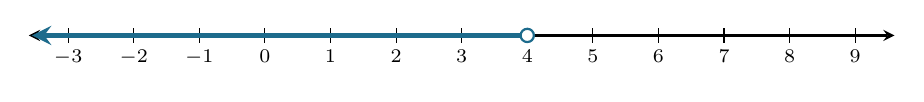
\begin{tikzpicture}[x=0.833cm, baseline=-1mm]\draw[thick,<->,>=stealth] (-3.6,0) -- (9.6,0);\foreach \k in {-3,...,9} \draw (\k,0.09) -- (\k,-0.09);\foreach \k in {-3,...,9} \node[below=-1pt, font=\scriptsize] at (\k,-0.09) {$\k$};\draw[accent, line width=2pt, ->, >=stealth] (4,0) -- (-3.55,0);\draw[accent, thick, fill=white] (4,0) circle (2.4pt);\end{tikzpicture}\par\vspace{2mm}

\textbf{2.} $3(x - 1) \ge  6$ \quad $\Rightarrow$ \quad $x - 1 \ge  2$ \quad $\Rightarrow$ \quad $x \ge  3$ \quad (filled circle, arrow right)\par
\hspace*{6mm}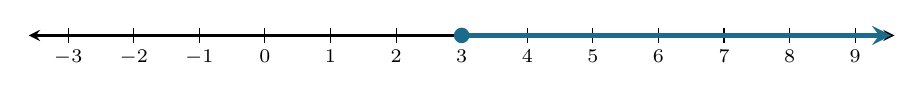
\begin{tikzpicture}[x=0.833cm, baseline=-1mm]\draw[thick,<->,>=stealth] (-3.6,0) -- (9.6,0);\foreach \k in {-3,...,9} \draw (\k,0.09) -- (\k,-0.09);\foreach \k in {-3,...,9} \node[below=-1pt, font=\scriptsize] at (\k,-0.09) {$\k$};\draw[accent, line width=2pt, ->, >=stealth] (3,0) -- (9.55,0);\draw[accent, thick, fill=accent] (3,0) circle (2.4pt);\end{tikzpicture}\par\vspace{2mm}

\textbf{3.} $5 - 2x \le  11$ \quad $\Rightarrow$ \quad $-2x \le  6$ \quad $\Rightarrow$ \quad $x \ge  -3$ \quad (divided by $-2$, so \textbf{flip}!)\par
\hspace*{6mm}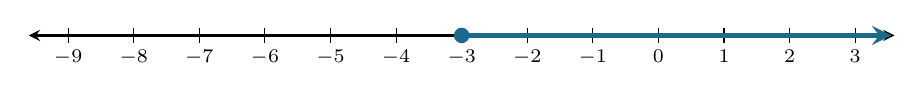
\begin{tikzpicture}[x=0.833cm, baseline=-1mm]\draw[thick,<->,>=stealth] (-9.6,0) -- (3.6,0);\foreach \k in {-9,...,3} \draw (\k,0.09) -- (\k,-0.09);\foreach \k in {-9,...,3} \node[below=-1pt, font=\scriptsize] at (\k,-0.09) {$\k$};\draw[accent, line width=2pt, ->, >=stealth] (-3,0) -- (3.55,0);\draw[accent, thick, fill=accent] (-3,0) circle (2.4pt);\end{tikzpicture}

\begin{rememberbox}
Check with a test number. For $x \ge  -3$, try $x = 0$: $5 - 2 \times  0 = 5$, and $5 \le  11$ \cmark.
So numbers bigger than $-3$ work, and the arrow points right.
\end{rememberbox}

\newpage\normalsize
\banner{5}{Inequalities}{Practice}{accent}
{\large\textbf{Solve each inequality, then show the answer on the number line.}} {\color{muted}Show your working in each box.}\par\vspace{1mm}
\begin{tcbraster}[raster columns=2, raster column skip=4mm, raster row skip=3mm]
\pbox{1}{5.0cm}{{\Large $x + 4 > 7$}\par\vfill Answer:\ \ansline{0.4}\par\vspace{4mm}\centering 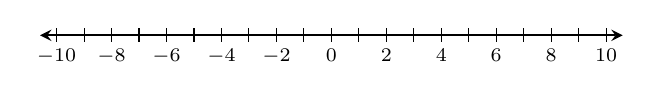
\begin{tikzpicture}[x=0.349cm, baseline=-1mm]\draw[thick,<->,>=stealth] (-10.6,0) -- (10.6,0);\foreach \k in {-10,...,10} \draw (\k,0.09) -- (\k,-0.09);\foreach \k in {-10,-8,...,10} \node[below=-1pt, font=\scriptsize] at (\k,-0.09) {$\k$};\end{tikzpicture}}
\pbox{2}{5.0cm}{{\Large $3x \le  12$}\par\vfill Answer:\ \ansline{0.4}\par\vspace{4mm}\centering 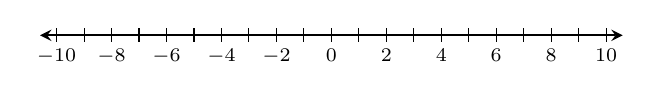
\begin{tikzpicture}[x=0.349cm, baseline=-1mm]\draw[thick,<->,>=stealth] (-10.6,0) -- (10.6,0);\foreach \k in {-10,...,10} \draw (\k,0.09) -- (\k,-0.09);\foreach \k in {-10,-8,...,10} \node[below=-1pt, font=\scriptsize] at (\k,-0.09) {$\k$};\end{tikzpicture}}
\pbox{3}{5.0cm}{{\Large $2x - 5 < 7$}\par\vfill Answer:\ \ansline{0.4}\par\vspace{4mm}\centering 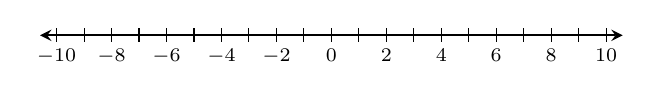
\begin{tikzpicture}[x=0.349cm, baseline=-1mm]\draw[thick,<->,>=stealth] (-10.6,0) -- (10.6,0);\foreach \k in {-10,...,10} \draw (\k,0.09) -- (\k,-0.09);\foreach \k in {-10,-8,...,10} \node[below=-1pt, font=\scriptsize] at (\k,-0.09) {$\k$};\end{tikzpicture}}
\pbox{4}{5.0cm}{{\Large $4x + 3 \ge  -9$}\par\vfill Answer:\ \ansline{0.4}\par\vspace{4mm}\centering 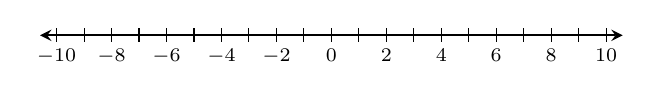
\begin{tikzpicture}[x=0.349cm, baseline=-1mm]\draw[thick,<->,>=stealth] (-10.6,0) -- (10.6,0);\foreach \k in {-10,...,10} \draw (\k,0.09) -- (\k,-0.09);\foreach \k in {-10,-8,...,10} \node[below=-1pt, font=\scriptsize] at (\k,-0.09) {$\k$};\end{tikzpicture}}
\pbox{5}{5.0cm}{{\Large $\frac{x}{2} + 1 > 3$}\par\vfill Answer:\ \ansline{0.4}\par\vspace{4mm}\centering 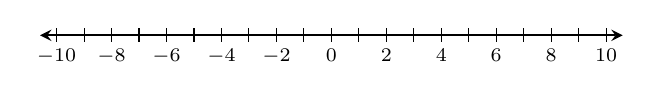
\begin{tikzpicture}[x=0.349cm, baseline=-1mm]\draw[thick,<->,>=stealth] (-10.6,0) -- (10.6,0);\foreach \k in {-10,...,10} \draw (\k,0.09) -- (\k,-0.09);\foreach \k in {-10,-8,...,10} \node[below=-1pt, font=\scriptsize] at (\k,-0.09) {$\k$};\end{tikzpicture}}
\pbox{6}{5.0cm}{{\Large $3(x - 2) \le  9$}\par\vfill Answer:\ \ansline{0.4}\par\vspace{4mm}\centering 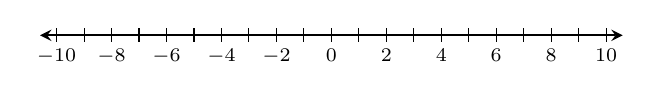
\begin{tikzpicture}[x=0.349cm, baseline=-1mm]\draw[thick,<->,>=stealth] (-10.6,0) -- (10.6,0);\foreach \k in {-10,...,10} \draw (\k,0.09) -- (\k,-0.09);\foreach \k in {-10,-8,...,10} \node[below=-1pt, font=\scriptsize] at (\k,-0.09) {$\k$};\end{tikzpicture}}
\pbox{7}{5.0cm}{{\Large $5 - x < 2$}\par\vfill Answer:\ \ansline{0.4}\par\vspace{4mm}\centering 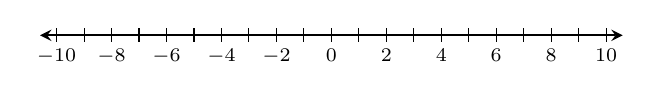
\begin{tikzpicture}[x=0.349cm, baseline=-1mm]\draw[thick,<->,>=stealth] (-10.6,0) -- (10.6,0);\foreach \k in {-10,...,10} \draw (\k,0.09) -- (\k,-0.09);\foreach \k in {-10,-8,...,10} \node[below=-1pt, font=\scriptsize] at (\k,-0.09) {$\k$};\end{tikzpicture}}
\pbox{8}{5.0cm}{{\Large $-2x + 1 \ge  7$}\par\vfill Answer:\ \ansline{0.4}\par\vspace{4mm}\centering 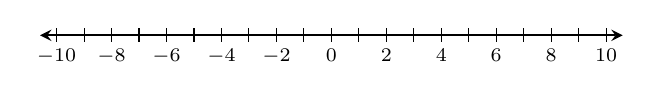
\begin{tikzpicture}[x=0.349cm, baseline=-1mm]\draw[thick,<->,>=stealth] (-10.6,0) -- (10.6,0);\foreach \k in {-10,...,10} \draw (\k,0.09) -- (\k,-0.09);\foreach \k in {-10,-8,...,10} \node[below=-1pt, font=\scriptsize] at (\k,-0.09) {$\k$};\end{tikzpicture}}
\end{tcbraster}
\vfill\centerline{\color{good}\bfseries \ding{51}\ Check your answers at the back. Fix any you got wrong.}
\newpage
\banner{6}{Writing Linear Rules}{Learn}{accent}
\begin{tcolorbox}[enhanced, colback=accentlight, colframe=accent, boxrule=0pt, leftrule=1.5mm, arc=0mm, top=1.5mm, bottom=1.5mm]\textbf{Goal:} I can write a rule like $y = 2x + 3$ from a table of values or a story\end{tcolorbox}
\large

A linear rule looks like $y = mx + c$.
\begin{itemize}[nosep]
\item $m$ is how much $y$ \textbf{changes} each time $x$ goes up by 1 (the \textbf{difference}).
\item $c$ is the value of $y$ when $x = 0$ (the \textbf{starting value}).
\end{itemize}

\begin{stepsbox}{From a table}
\begin{enumerate}[nosep]
\item Check $x$ goes up by 1 each time. Find the \textbf{difference} between the $y$ values: that's $m$.
\item Find $y$ when $x = 0$: that's $c$. If the table doesn't start at 0, \textbf{work backwards} one step at a time.
\item Write $y = mx + c$ and \textbf{check} it with another column.
\end{enumerate}
\end{stepsbox}

\begin{examples}
\example{\begin{tabular}{c|cccc}$x$&0&1&2&3\\\hline$y$&3&5&7&9\end{tabular}}{Goes up by 2: $m = 2$\\At $x = 0$, $y = 3$: $c = 3$}{$= y = 2x + 3$}
\example{\begin{tabular}{c|cccc}$x$&1&2&3&4\\\hline$y$&7&10&13&16\end{tabular}}{Goes up by 3: $m = 3$\\Back one step: $7 - 3 = 4$}{$= y = 3x + 4$}
\example{\begin{tabular}{c|cccc}$x$&0&1&2&3\\\hline$y$&10&8&6&4\end{tabular}}{Goes \textbf{down} by 2: $m = -2$\\At $x = 0$, $y = 10$}{$= y = -2x + 10$}
\end{examples}

\subsection*{From a story}
The \textbf{fixed amount} (a starting fee or starting value) is $c$. The amount \textbf{per} hour, week, km\ldots{} is $m$.
\begin{examples}
\example{\text{Gym}}{\$60 joining fee plus \$15 per week. Cost $C$ after $w$ weeks.}{$= C = 15w + 60$}
\example{\text{Candle}}{30 cm tall, burns down 2 cm every hour. Height $h$ after $t$ hours.}{$= h = 30 - 2t$}
\example{\text{Phone}}{\$20 a month plus \$5 per GB of data. Cost $C$ for $g$ GB.}{$= C = 5g + 20$}
\end{examples}

\newpage\normalsize
\banner{6}{Writing Linear Rules}{Practice}{accent}
{\large\textbf{Write the rule for each table. For the stories, write an equation.}} {\color{muted}Show your working in each box.}\par\vspace{1mm}
\begin{tcbraster}[raster columns=2, raster column skip=4mm, raster row skip=3mm]
\pbox{1}{3.6cm}{\hspace{2mm}{\large\renewcommand{\arraystretch}{1.25}\begin{tabular}{|c|c|c|c|c|}\hline$x$ & 0 & 1 & 2 & 3 \\ \hline $y$ & 1 & 4 & 7 & 10 \\ \hline\end{tabular}}\par\vfill{\Large $y =$}\hspace{2mm}\ansline{0.75}}
\pbox{2}{3.6cm}{\hspace{2mm}{\large\renewcommand{\arraystretch}{1.25}\begin{tabular}{|c|c|c|c|c|}\hline$x$ & 0 & 1 & 2 & 3 \\ \hline $y$ & 5 & 7 & 9 & 11 \\ \hline\end{tabular}}\par\vfill{\Large $y =$}\hspace{2mm}\ansline{0.75}}
\pbox{3}{3.6cm}{\hspace{2mm}{\large\renewcommand{\arraystretch}{1.25}\begin{tabular}{|c|c|c|c|c|}\hline$x$ & 1 & 2 & 3 & 4 \\ \hline $y$ & 6 & 10 & 14 & 18 \\ \hline\end{tabular}}\par\vfill{\Large $y =$}\hspace{2mm}\ansline{0.75}}
\pbox{4}{3.6cm}{\hspace{2mm}{\large\renewcommand{\arraystretch}{1.25}\begin{tabular}{|c|c|c|c|c|}\hline$x$ & 1 & 2 & 3 & 4 \\ \hline $y$ & 2 & 7 & 12 & 17 \\ \hline\end{tabular}}\par\vfill{\Large $y =$}\hspace{2mm}\ansline{0.75}}
\pbox{5}{3.6cm}{\hspace{2mm}{\large\renewcommand{\arraystretch}{1.25}\begin{tabular}{|c|c|c|c|c|}\hline$x$ & 0 & 1 & 2 & 3 \\ \hline $y$ & 12 & 9 & 6 & 3 \\ \hline\end{tabular}}\par\vfill{\Large $y =$}\hspace{2mm}\ansline{0.75}}
\pbox{6}{3.6cm}{\hspace{2mm}{\large\renewcommand{\arraystretch}{1.25}\begin{tabular}{|c|c|c|c|c|}\hline$x$ & 2 & 3 & 4 & 5 \\ \hline $y$ & 1 & 3 & 5 & 7 \\ \hline\end{tabular}}\par\vfill{\Large $y =$}\hspace{2mm}\ansline{0.75}}
\pbox[raster multicolumn=2]{7}{3.0cm}{{\large An electrician charges a \$70 call-out fee plus \$45 per hour. Write an equation for the total cost $C$ of a job that takes $h$ hours.}\par\vfill\ansline{0.95}}
\pbox[raster multicolumn=2]{8}{3.0cm}{{\large A taxi charges \$3.50 to start, plus \$2 per kilometre. Write an equation for the fare $F$ for a trip of $d$ kilometres.}\par\vfill\ansline{0.95}}
\pbox[raster multicolumn=2]{9}{3.0cm}{{\large A water tank holds 200 litres and leaks 5 litres every hour. Write an equation for the amount of water $W$ left after $t$ hours.}\par\vfill\ansline{0.95}}
\end{tcbraster}
\vfill\centerline{\color{good}\bfseries \ding{51}\ Check your answers at the back. Fix any you got wrong.}
\newpage
\banner{\ding{51}}{Skill Checks}{Teacher marks}{checkcol}
{\large Name: \fillline{8cm}}\hfill\par\vspace{1mm}
Do these \textbf{on your own --- no notes}. Show your working, and write your final answer on the line.
\checkhead{1}{Factorising Fully}{Factorise fully.}{4}
\begin{tcbraster}[raster columns=4, raster column skip=3mm]
\cbox{1}{$15x + 45$}{4.4cm}
\cbox{2}{$24a - 36$}{4.4cm}
\cbox{3}{$8x^{2} + 20x$}{4.4cm}
\cbox{4}{$18xy - 12x$}{4.4cm}
\end{tcbraster}
\checkhead{2}{Substituting Negatives}{Find the value.}{4}
\begin{tcbraster}[raster columns=4, raster column skip=3mm]
\cbox{1}{$5x + 3$\\[1pt]{\normalsize when $x = -2$}}{4.4cm}
\cbox{2}{$a - b$\\[1pt]{\normalsize when $a = -4$, $b = -6$}}{4.4cm}
\cbox{3}{$x^{2} - 4x$\\[1pt]{\normalsize when $x = -3$}}{4.4cm}
\cbox{4}{$2ab$\\[1pt]{\normalsize when $a = -5$, $b = 3$}}{4.4cm}
\end{tcbraster}
\checkhead{3}{Index Laws}{Simplify, and explain.}{3}
\begin{tcbraster}[raster columns=4, raster column skip=3mm]
\cbox{1}{$2^{5} \times  2^{3}$}{5.7cm}
\cbox{2}{$12x^{7} \div  3x^{2}$}{5.7cm}
\kbox[raster multicolumn=2]{3}{5.7cm}{{\normalsize Ana says $4^{3} \times  4^{5} = 16^{8}$ because $4 \times  4 = 16$ and $3 + 5 = 8$. Explain why Ana is wrong. State the index law and give the correct answer.}\par\vfill\par\vspace{5mm}\ansline{1}\par\vspace{5mm}\ansline{1}\par\vspace{5mm}\ansline{1}}
\end{tcbraster}
\newpage
\banner{\ding{51}}{Skill Checks}{Continued}{checkcol}
{\large Name: \fillline{8cm}}\hfill\fcolorbox{checkcol}{white}{\parbox[c][8mm][c]{4.2cm}{\centering\color{checkcol}\bfseries\large Total: \underline{\hspace{9mm}} / 18}}\par\vspace{1mm}
Do these \textbf{on your own --- no notes}. Show your working, and write your final answer on the line.
\checkhead{4}{Equations with Brackets}{Solve.}{3}
\begin{tcbraster}[raster columns=4, raster column skip=3mm]
\kbox{1}{5.6cm}{{\large $3(x - 4) = 18$}\par\vfill{\large $x =$}\hspace{2mm}\ansline{0.7}}
\kbox{2}{5.6cm}{{\large $4(2x + 3) = 4$}\par\vfill{\large $x =$}\hspace{2mm}\ansline{0.7}}
\kbox[raster multicolumn=2]{3}{5.6cm}{{\normalsize Tama thinks of a number, adds 7, then multiplies by 3. The answer is 39. Write an equation and solve it.}\par\vfill Equation:\ \ansline{0.7}\par\vspace{4mm}Answer:\ \ansline{0.4}}
\end{tcbraster}
\checkhead{5}{Inequalities}{Solve, then show on the number line.}{2}
\begin{tcbraster}[raster columns=4, raster column skip=3mm]
\kbox[raster multicolumn=2]{1}{5.6cm}{{\large $3x - 4 > 8$}\par\vfill Answer:\ \ansline{0.4}\par\vspace{4mm}\centering 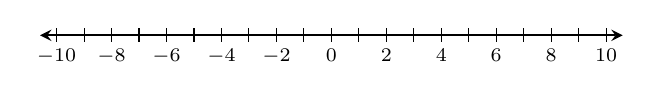
\begin{tikzpicture}[x=0.349cm, baseline=-1mm]\draw[thick,<->,>=stealth] (-10.6,0) -- (10.6,0);\foreach \k in {-10,...,10} \draw (\k,0.09) -- (\k,-0.09);\foreach \k in {-10,-8,...,10} \node[below=-1pt, font=\scriptsize] at (\k,-0.09) {$\k$};\end{tikzpicture}}
\kbox[raster multicolumn=2]{2}{5.6cm}{{\large $6 - 2x \le  10$}\par\vfill Answer:\ \ansline{0.4}\par\vspace{4mm}\centering 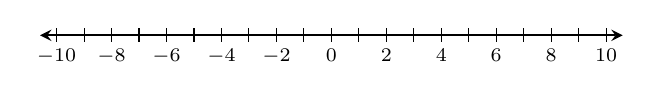
\begin{tikzpicture}[x=0.349cm, baseline=-1mm]\draw[thick,<->,>=stealth] (-10.6,0) -- (10.6,0);\foreach \k in {-10,...,10} \draw (\k,0.09) -- (\k,-0.09);\foreach \k in {-10,-8,...,10} \node[below=-1pt, font=\scriptsize] at (\k,-0.09) {$\k$};\end{tikzpicture}}
\end{tcbraster}
\checkhead{6}{Writing Linear Rules}{Write the rule.}{2}
\begin{tcbraster}[raster columns=4, raster column skip=3mm]
\kbox[raster multicolumn=2]{1}{5.6cm}{\hspace{2mm}{\large\renewcommand{\arraystretch}{1.25}\begin{tabular}{|c|c|c|c|c|}\hline$x$ & 1 & 2 & 3 & 4 \\ \hline $y$ & 1 & 4 & 7 & 10 \\ \hline\end{tabular}}\par\vfill{\large $y =$}\hspace{2mm}\ansline{0.75}}
\kbox[raster multicolumn=2]{2}{5.6cm}{{\normalsize A school trip costs \$200 for the bus plus \$12 per student. Write an equation for the total cost $C$ when $n$ students go.}\par\vfill\ansline{0.95}}
\end{tcbraster}
\newpage
\setlength{\multicolsep}{3pt plus 1pt}\titlespacing*{\subsection}{0pt}{6pt}{2pt}
{\LARGE\bfseries\color{accent} Answers to the Practice Questions}\par\vspace{1mm}
{\small\color{muted} Terms can be in a different order and still be right --- e.g. $2b + 3a$ is the same as $3a + 2b$.}\par
\subsection*{1. Factorising Fully}
\textbf{\color{muted}}
\begin{multicols}{4}\begin{enumerate}[nosep, label=\arabic*., start=1]
\item $10(x + 3)$
\item $8(2a - 3)$
\item $9(2y + 3)$
\item $12(2x - 3)$
\item $10(2m + 5)$
\item $14(3 - 2x)$
\item $x(x + 9)$
\item $3x(2x + 3)$
\item $5a(2a - 3)$
\item $8x(2x + 3)$
\item $3a(3b + 4)$
\item $10y(2x - 3)$
\end{enumerate}\end{multicols}

\subsection*{2. Substituting Negatives}
\textbf{\color{muted}}
\begin{multicols}{4}\begin{enumerate}[nosep, label=\arabic*., start=1]
\item $5$
\item $-20$
\item $9$
\item $-2$
\item $36$
\item $-14$
\item $10$
\item $11$
\item $-2$
\item $18$
\item $11$
\item $5$
\end{enumerate}\end{multicols}

\subsection*{3. Index Laws}
\begin{multicols}{4}\begin{enumerate}[nosep, label=\arabic*., start=1]
\item $5^{7}$
\item $x^{8}$
\item $7^{6}$
\item $a^{6}$
\item $x^{12}$
\item $12x^{7}$
\item $4a^{5}$
\item $9x^{4}$
\end{enumerate}\end{multicols}
\begin{enumerate}[nosep, label=\arabic*., start=9]
\item When multiplying powers with the same base, keep the base and add the indices: $a^m \times  a^n = a^{m+n}$. The base stays 2, so $2^{3} \times  2^{4} = 2^{7}$ ($= 128$), not $4^{7}$.
\item When dividing powers with the same base, keep the base and subtract the indices: $a^m \div  a^n = a^{m-n}$. The base stays 5, so $5^{8} \div  5^{2} = 5^{6}$, not $1^{4}$.
\end{enumerate}

\subsection*{4. Equations with Brackets}
\begin{multicols}{4}\begin{enumerate}[nosep, label=\arabic*., start=1]
\item $x = 4$
\item $x = 9$
\item $x = 4$
\item $x = -3$
\item $x = 2$
\item $x = 3.5$
\end{enumerate}\end{multicols}
\begin{enumerate}[nosep, label=\arabic*., start=7]
\item $5(n - 3) = 40$, so $n = 11$
\item $4(x + 6) = 52$, so $x = 7$
\item $5(t + 3) = 85$, so $t = 14$
\end{enumerate}

\subsection*{5. Inequalities}
\begin{multicols}{2}\begin{enumerate}[nosep, label=\arabic*., start=1]
\item $x > 3$\quad 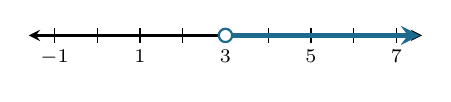
\begin{tikzpicture}[x=0.543cm, baseline=-1mm]\draw[thick,<->,>=stealth] (-1.6,0) -- (7.6,0);\foreach \k in {-1,...,7} \draw (\k,0.09) -- (\k,-0.09);\foreach \k in {-1,1,...,7} \node[below=-1pt, font=\scriptsize] at (\k,-0.09) {$\k$};\draw[accent, line width=2pt, ->, >=stealth] (3,0) -- (7.55,0);\draw[accent, thick, fill=white] (3,0) circle (2.4pt);\end{tikzpicture}
\item $x \le  4$\quad 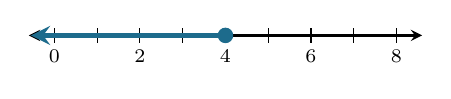
\begin{tikzpicture}[x=0.543cm, baseline=-1mm]\draw[thick,<->,>=stealth] (-0.6,0) -- (8.6,0);\foreach \k in {0,...,8} \draw (\k,0.09) -- (\k,-0.09);\foreach \k in {0,2,...,8} \node[below=-1pt, font=\scriptsize] at (\k,-0.09) {$\k$};\draw[accent, line width=2pt, ->, >=stealth] (4,0) -- (-0.55,0);\draw[accent, thick, fill=accent] (4,0) circle (2.4pt);\end{tikzpicture}
\item $x < 6$\quad 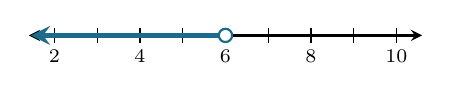
\begin{tikzpicture}[x=0.543cm, baseline=-1mm]\draw[thick,<->,>=stealth] (1.4,0) -- (10.6,0);\foreach \k in {2,...,10} \draw (\k,0.09) -- (\k,-0.09);\foreach \k in {2,4,...,10} \node[below=-1pt, font=\scriptsize] at (\k,-0.09) {$\k$};\draw[accent, line width=2pt, ->, >=stealth] (6,0) -- (1.45,0);\draw[accent, thick, fill=white] (6,0) circle (2.4pt);\end{tikzpicture}
\item $x \ge  -3$\quad 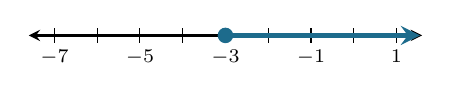
\begin{tikzpicture}[x=0.543cm, baseline=-1mm]\draw[thick,<->,>=stealth] (-7.6,0) -- (1.6,0);\foreach \k in {-7,...,1} \draw (\k,0.09) -- (\k,-0.09);\foreach \k in {-7,-5,...,1} \node[below=-1pt, font=\scriptsize] at (\k,-0.09) {$\k$};\draw[accent, line width=2pt, ->, >=stealth] (-3,0) -- (1.55,0);\draw[accent, thick, fill=accent] (-3,0) circle (2.4pt);\end{tikzpicture}
\item $x > 4$\quad 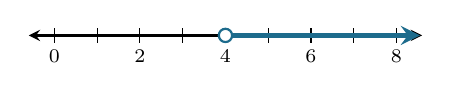
\begin{tikzpicture}[x=0.543cm, baseline=-1mm]\draw[thick,<->,>=stealth] (-0.6,0) -- (8.6,0);\foreach \k in {0,...,8} \draw (\k,0.09) -- (\k,-0.09);\foreach \k in {0,2,...,8} \node[below=-1pt, font=\scriptsize] at (\k,-0.09) {$\k$};\draw[accent, line width=2pt, ->, >=stealth] (4,0) -- (8.55,0);\draw[accent, thick, fill=white] (4,0) circle (2.4pt);\end{tikzpicture}
\item $x \le  5$\quad 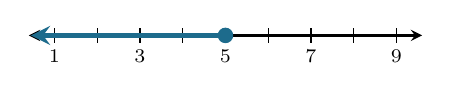
\begin{tikzpicture}[x=0.543cm, baseline=-1mm]\draw[thick,<->,>=stealth] (0.4,0) -- (9.6,0);\foreach \k in {1,...,9} \draw (\k,0.09) -- (\k,-0.09);\foreach \k in {1,3,...,9} \node[below=-1pt, font=\scriptsize] at (\k,-0.09) {$\k$};\draw[accent, line width=2pt, ->, >=stealth] (5,0) -- (0.45,0);\draw[accent, thick, fill=accent] (5,0) circle (2.4pt);\end{tikzpicture}
\item $x > 3$\quad 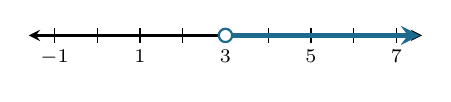
\begin{tikzpicture}[x=0.543cm, baseline=-1mm]\draw[thick,<->,>=stealth] (-1.6,0) -- (7.6,0);\foreach \k in {-1,...,7} \draw (\k,0.09) -- (\k,-0.09);\foreach \k in {-1,1,...,7} \node[below=-1pt, font=\scriptsize] at (\k,-0.09) {$\k$};\draw[accent, line width=2pt, ->, >=stealth] (3,0) -- (7.55,0);\draw[accent, thick, fill=white] (3,0) circle (2.4pt);\end{tikzpicture}
\item $x \le  -3$\quad 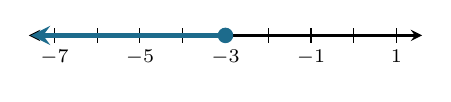
\begin{tikzpicture}[x=0.543cm, baseline=-1mm]\draw[thick,<->,>=stealth] (-7.6,0) -- (1.6,0);\foreach \k in {-7,...,1} \draw (\k,0.09) -- (\k,-0.09);\foreach \k in {-7,-5,...,1} \node[below=-1pt, font=\scriptsize] at (\k,-0.09) {$\k$};\draw[accent, line width=2pt, ->, >=stealth] (-3,0) -- (-7.55,0);\draw[accent, thick, fill=accent] (-3,0) circle (2.4pt);\end{tikzpicture}
\end{enumerate}\end{multicols}

\subsection*{6. Writing Linear Rules}
\begin{multicols}{4}\begin{enumerate}[nosep, label=\arabic*., start=1]
\item $y = 3x + 1$
\item $y = 2x + 5$
\item $y = 4x + 2$
\item $y = 5x - 3$
\item $y = -3x + 12$
\item $y = 2x - 3$
\item $C = 45h + 70$
\item $F = 2d + 3.5$
\item $W = 200 - 5t$
\end{enumerate}\end{multicols}

\end{document}
